\documentclass[../main.tex]{subfiles}
\graphicspath{{\subfix{../imagenes/}}}

\begin{document}

\chapter{Methodology} \label{chap:methodology}

 In the previous chapter, we made a thorough high-level definition of the functionalities that the platform we propose has, even formalizing each of the components that comprise the system and the adaptive tactics we have selected to implement in our solution.

 This chapter aims to delve deeper into the methodology we employed to implement these functionalities and tactics for their application to TB detection. We'll discuss the specific technologies that we applied, the machine learning models used, the processing of the data used, training and evaluation processes, and the methodology we propose to evaluate the use of adaptation techniques with the data in this platform, the results from that evaluation are reported in the next chapter.

\vspace{-0.2cm}
 \section{Tools Used}
    \vspace{-0.3cm}
    \subsection{Programming Languages}

    The main programming language used in this work is \textbf{Python}, which is a high-level, general-purpose programming language that is widely used in the field of machine learning and data science due to its wide ecosystem of libraries and frameworks that facilitate the development of machine learning models and applications.

    Additionally, we used \textbf{SQL}, a query language used to interact with relational databases, to interact with the Knowledge Database that we implemented (see section \ref{sec:knowledge_db}). This included making queries to get data from the database and creating new objects and tables, among other database operations.

    \subsection{Frameworks and Libraries}

    We proceed by listing some of the most relevant frameworks and libraries we used to build the components and implement the experiments described in this work. These tools were selected based on their popularity, ease of use, and documentation and helped us speed up the development process significantly.

    \vspace{0.5cm}
    
    \begin{enumerate}
        \item \textbf{PyTorch and TensorFlow} \cite{pytorch, tensorflow2015} were the two frameworks used to develop, train, and/or evaluate all the deep learning models for this work. They are the most popular and widely used libraries for developing DL models. We used PyTorch for most of the experiments and models trained and TensorFlow for some of the ones that required the use of specific models that were only implemented in that framework. 
        % Both PyTorch and TensorFlow are implemented in Python.
        \item \textbf{Numpy and Pandas} \cite{numpy, pandas}: Numpy is a scientific library in Python that supports mathematical operations with multi-dimensional arrays and matrices. Pandas built on top of Numpy the easy data structures for easy data manipulation. We used both of these libraries extensively for data processing and writing augmentation tasks.
        \item \textbf{PostgreSQL \cite{postgresql}}: As we mentioned earlier, we used PostgreSQL to implement the database where we stored the data, annotations, and other information needed by the system.  PostgreSQL is an open-source Object-Relational Database Management System (ORDBMS) that is very popular and widely used in the industry.
        \item \textbf{Streamlit} \cite{streamlit} is an open-source framework for building web applications in Python. We used it to design and implement the labeling interface that we used to annotate the data (see section \ref{sec:labeling_interface}). The interface was designed to be simple, intuitive to use and responsive to work on mobile devices. Streamlit allowed us to easily integrate the interface with the rest of the system, making it a great choice for this task.
        \item \textbf{MLFlow \cite{mlflow}}, an open-source platform and Python framework for tracking ML models and experiments, was used as a means to implement our model repository. We used this platform to store our ML models and their associated metadata.
    \end{enumerate}
    \vspace{-0.4cm}
    Other tools we worked with throughout the implementation of this project included \textbf{Docker \cite{docker}}, a virtualization platform we used to package the different components of our system and ensure a consistent development environment, \textbf{FastAPI \cite{fastapi}} for implementing the APIs that allowed communication between components, as well as a number of other tools for analysis, visualization, and image processing \cite{matplotlib, scikit-learn, opencv}. 

    \vspace{-0.5cm}

    \subsection{Hardware}
    \vspace{-0.5cm}
    
    All the methods were implemented and tested on a personal MacBook Pro (2021) with an M1 Pro chip, 16GB of RAM, and 1TB of SSD storage. Most of the ML training and evaluation experiments were also done with this device. 
    
    Additionally, we used the Google Colab platform \footnote{\url{https://colab.research.google.com/}} to get access to NVIDIA GPUs in the cloud, which was used to train the ML models that were too big (or too slow) to attempt to do so locally. In order to share code/data between the local and cloud environments, we used Google Drive \footnote{\url{https://www.google.com/intl/en-GB/drive/}} and GitHub \footnote{\url{https://github.com}}. 
    
    We list some of the GPUs we had available in the Colab platform along with their VRAM capacity and performance in the table below \footnote{See \url{hhttps://resources.nvidia.com/l/en-us-gpu} for more information}:

    \begin{table}[h]
        \centering
        \begin{tabular}{l|l|l}
        \toprule
        \textbf{GPU} & \textbf{VRAM} & \textbf{FP32 Performance} \\
        \midrule
        T4 & 16GB & 8 TFLOPs \\
        V100 & 16GB & 14 TFLOPs \\
        A100 & 40GB & 19.5 TFLOPs \\
        \bottomrule
        \end{tabular}
        \caption{Hardware specifications of different Nvidia Tesla GPUs available in Google Colab}
        \label{table:tesla_models}
\end{table}

    \vspace{-0.3cm}

    Note VRAM capacity is important because it limits the size of the models that can be trained on a given GPU and FP32 performance measures the number of floating-point operations that can be performed per second, which largely determines how long it takes to train a model.. 
    
    For example, the DETR model we used in our experiments (see section \ref{sec:detr}) requires at least 12GB of VRAM to be trained in its default configuration and up to 25GB of VRAM with the configurations that theoretically allow it to detect smaller objects better (DETR-DCN).

    FP32 performance measures the number of floating-point operations that can be performed per second, which largely determines how long it takes to train a model. Since the cost of V100 and A100 GPUs was significantly higher than that of the T4s (which could sometimes be used for free in Colab), we only used them sparingly for the more demanding experiments. 
 
 
 \section{Data Source and Selection}

    The dataset used in this work to train the models and evaluate the performance of the proposed system was sourced from Kaggle, a popular platform for data science competitions and sharing datasets and ML notebooks \cite{kaggle}.  
    
    The dataset \footnote{\url{https://www.kaggle.com/datasets/saife245/tuberculosis-image-datasets}} consists of 928 images of sputum smear microscopy along with the annotated bounding boxes at the regions where TB Bacilli is localized for a total of 3,734 ground-truth annotations. The original collection of this data was carried out through specialized software and hardware for collecting samples from sputum. A Gram stain was typically performed to identify the bacteria causing the infection \cite{tbbacillus_kaggle_dataset}.

    This data is of high relevance to our work and gives us the opportunity to train our model effectively on real-world data. Figure \ref{fig:tbbacillus_image_examples} shows some examples of the images in this dataset with their corresponding annotations.

    To select the data used for training, validation, and testing of the models, we used the same methods as Visuña et al. \cite{visuna_novel_2023} (the same dataset we used in this work), which only includes the images that were deemed more reliable and whose annotations seemed to be more accurate and consistent with domain experts.

    With this, approximately only 30\% of the total amount of images met the criteria for being selected. The rest of the images were discarded because they were either too blurry, had too many artifacts, or had annotations that were deemed too inconsistent (mainly due to missing annotations).

    The final dataset used for training and testing the models is summarized in table \ref{tab:training-test-data}.

 
    \begin{figure}[ht]
     \centering
     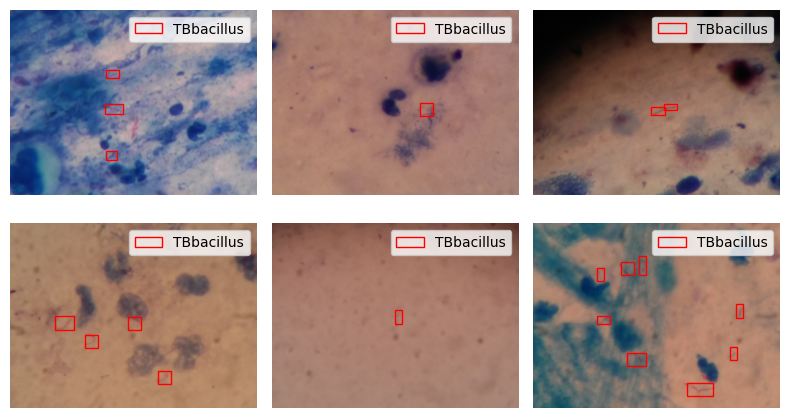
\includegraphics[width=0.93\linewidth]{figures/tbbacilus-dataset.png}
     \caption{Example of some smear-sputum microscopy images in the dataset. Boxes show the presence of TB Bacilli }
     \label{fig:tbbacillus_image_examples}
 \end{figure}

 %  202 training images 1467 annotations
% 40 validation images 235 annotations
% 66 test images 351 annotations
 
 %  Table of training and test data
 \begin{table}[h]
    \centering
    \caption{Training and Test Data}
    \label{tab:training-test-data}
    \begin{tabular}{l|c|c}
        \toprule
        \textbf{Subset} & \textbf{Number of Images} & \textbf{Number of Annotations} \\
        \midrule
        \textbf{Training} & 202 & 1467 \\
        \textbf{Validation} & 40 & 235 \\
        \textbf{Test} & 66 & 351 \\
        \midrule
        \textbf{Total} & 308 & 2053 \\
        % \textbf{TB Bacillus (Augmented)} & 2000 & 1600 & 400 \\
        % \textbf{TB Bacillus (Augmented + Balanced)} & 4000 & 3200 & 800 \\
        \bottomrule
    \end{tabular}
\end{table}

\vspace{-0.6cm}
 \section{ML model Training and Evaluation}
\vspace{-0.4cm}

 The data mentioned above was used to train a baseline object detection model to detect regions in the images where TB bacilli is localized. The training and validation subsets were used during the model training process while the \textit{test} subset was assumed to be unseen data and was used to evaluate the final performance of the model.

 The idea is that this baseline model could be used to compare the performance of the system with and without the adaptive tactics we implemented. Other models were also trained using different data subsets and hyperparameter configurations depending on the technique being evaluated and compared with this one. In section \ref{sec:adaptive_experiments}, we discuss the details of the experiments we conducted and the models we trained.

 The deep learning model that we chose to train for this task was DETR (Detection Transformer) \cite{carionEndtoEndObjectDetection2020}, an end-to-end computer vision model that was introduced in 2020 by researchers at Meta AI. \footnote{We originally considered using the same Nas-Net Mobile model used in \cite{visuna_novel_2023}. As we've established, this model was trained on the same dataset we used. However, we found that the inference speed of this model was too slow for the workflows we wanted to evaluate, and its performance was not significantly better than that of DETR. We show the performance of this model compared to our model in chapter \ref{chap:results}.}

 DETR leverages the transformer architecture \cite{vaswaniAttentionAllYou2017}, widely recognized for its prevalent use in natural language processing tasks, and extends its use to the CV domain. The model discards complex pipeline mechanisms such as non-maximum suppression used in object detectors like Faster R-CNN (see section \ref{sec:computer_vision_sota} in the state-of-the-art chapter) and operates end-to-end, treating object detection as a direct set prediction problem.

 \begin{figure}[t]
     \centering
     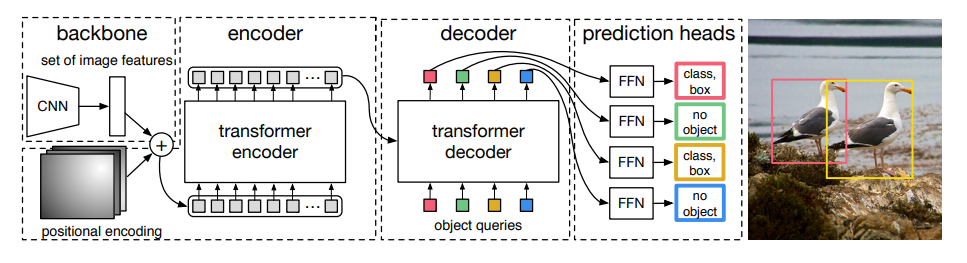
\includegraphics[width=1.1\linewidth]{figures/detr_architecture.png}
     \caption{
        Architecture of DETR from \cite{carionEndtoEndObjectDetection2020}. 
        \footnotesize The model first computes a set of image features from a CNN backbone and a set of positional encodings that are used to encode the spatial information of the image. Then, the model uses a transformer encoder to process the image features and positional encodings and a transformer decoder to generate a set of object queries that are used to predict the bounding boxes and class labels of the objects in the image.
     }
     \label{fig:detr-architecture}
 \end{figure}

 The specific version of DETR that we used was one open-sourced by Facebook Research through Github that is officially available in the Pytorch model Hub \footnote{\url{https://github.com/facebookresearch/detr}}. This model uses a ResNet-50 model as backbone \cite{heSpatialPyramidPooling2014} and was pre-trained on the COCO dataset \cite{linMicrosoftCOCOCommon2015}. 

\vspace{-0.4cm}
\subsection{Training Process}
 \vspace{-0.3cm}
 
 Thus, we proceeded to fine-tune this pre-trained model on our selected dataset. Our training script was adapted from the one included in their official repository but modified to directly pull the data from our database that was specifically tagged to be used for training. We also modified the script to use the hyperparameters that we selected.

 Since the original code was written to train the model with the COCO dataset, we had to adapt it to work with our data. This included creating our own data loading mechanisms that grab the relevant images from the database and apply the necessary transformations, which for DETR included resizing the images to 800x1333 pixels, normalizing them to $[0, 1]$, and converting them to PyTorch tensors in the same output format as COCO. 

 While the original paper includes the training-time data augmentations of randomly cropping a part of the image and applying color jittering (randomly changing the brightness, contrast, saturation, and hue of the image), we realized these augmentations wouldn't be suitable to our data.  
 
 The reason for that is that - unlike the objects in COCO - the individual bacilli in our images were very small and spread apart. Because of that, the cropping technique would more often than not crop out and leave only a part of the image with no bacilli in it, making it impossible for the model to learn to detect them. 
 
 % Additionally, since the size of the bacilli in microscopy images doesn't change much from image to image, this kind of technique is unlikely to benefit our training. 
 We also decided to leave out the color jittering augmentation. According to the relevant literature (\cite{osman_tuberculosis_2011}), the color of the bacilli is a very important feature for their detection, and we didn't want to risk altering it.

Thus, the only augmentation we used from the original paper was doing a random horizontal flip to the image with a probability of 0.5 and resizing the image to different aspect ratios.

The training process was done in batches of 2 images, The model would detect 100 queries (i.e., objects) per image - the majority of which would be classified as background. The model was trained for 25 epochs with a learning rate of 0.0001 and a weight decay of 0.0001. Additionally, the learning rate was decayed by a factor of 0.1 at epochs 15 and 20 to improve the chances of convergence. 

The base model was trained on a single NVIDIA Tesla T4 GPU. Each full training run would usually take around 40 minutes with the entire dataset, and convergence generally occurred at around epoch 20.

We also trained a second version of the model with the same hyperparameters but added a dilation convolutional layer to the CNN backbone to increase its receptive field, a configuration (DETR-DC5) that the authors of the paper claimed improved the performance of DETR on small objects. This modification, however, increases the computational cost of the model by a factor of 2 \cite{carionEndtoEndObjectDetection2020}.

We trained this version on a single A100 GPU for 30 epochs, which took 15 minutes to fully train. We found that this version of the model initially achieves significantly lower validation losses but eventually converges to similar values as the regular one. 

Since the performance difference was not significant enough to justify the extra cost, we decided to use the first version for the rest of the experiments. Image \ref{fig:loss_plots_detr_base} shows the loss and class error of the two models throughout the training process. Figure \ref{fig:detr_base_true_pred_examples} shows some examples of the predictions made by the base model on the test set.

\begin{figure}[ht]
    \centering
    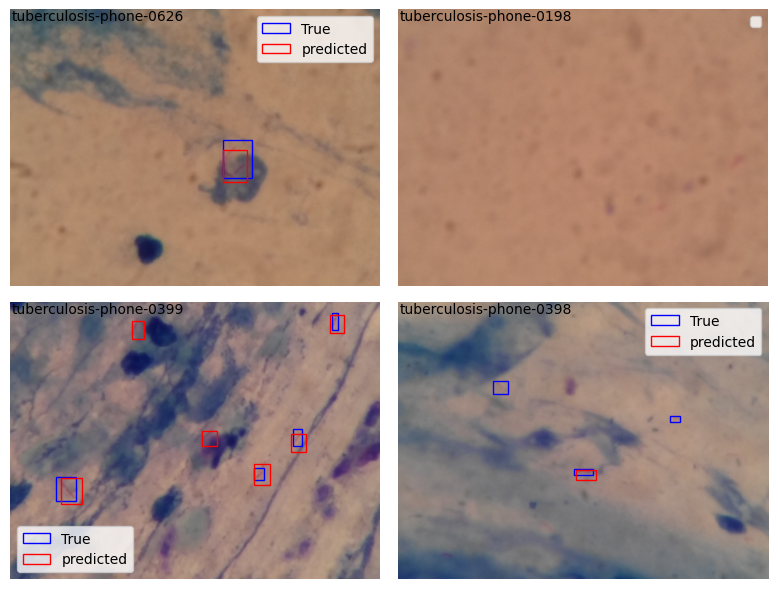
\includegraphics[width=0.65\linewidth]{figures/detr_base_true_pred_examples.png}
    \caption{Example of the predictions made by the DETR model on the test set. The blue boxes represent the ground truth annotations, while the red ones represent model predictions.}
    \label{fig:detr_base_true_pred_examples}
\end{figure}

\begin{figure}[ht]
    \centering
    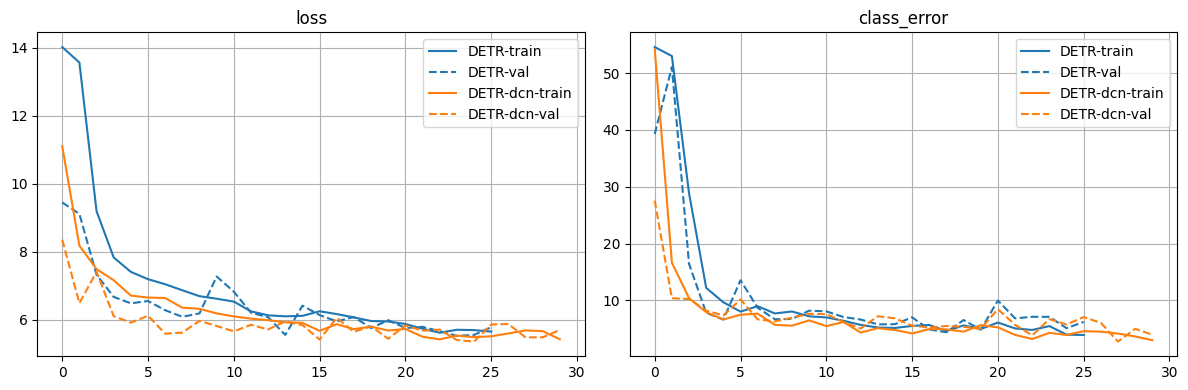
\includegraphics[width=1\linewidth]{figures/detr-base-loss-plots.png}
    \caption{Training and validation Loss of the DETR models and class errors after training each epoch. \footnotesize Class error refers to the accumulated error of classifying boxes as bacilli or background. DETR-DC5 is the model with a dilation layer.}
    \label{fig:loss_plots_detr_base}
\end{figure}


    
    \subsection{Performance Metrics}
        
    The metrics we report in the evaluation process are some of the common ones to report performance for object detection tasks: Average Precision (AP) and Average Recall (AR) at different intersections over union (IoU) thresholds. Which are also the ones used for COCO and in the DETR paper.

    The IoU is a measure of the overlap between bounding boxes. It is calculated as the area of overlap between the predicted bounding box and the ground truth bounding box divided by the area of the union of the two bounding boxes. Thus, when a single detection surpasses a certain IoU threshold, we consider it to be a true positive.

    Precision refers to the proportion of correct positive predictions out of 
    the \textit{total} predictions, while recall refers to the proportion of correct predictions out of \textit{actual} positives. 
    % Generally, precision is a good metric to use when we want to minimize the number of false positives, while recall is a good metric to use when we want to minimize the number of false negatives. 

    Generally, the IoU threshold is set to 0.5, meaning that if the IoU between the predicted and ground truth bounding boxes is greater than this number, the prediction is considered correct. We call these metrics AP@50 and AR@50, respectively. But while these two are the most common metrics to evaluate object detection models, we also report the performance of the models at an IoU threshold of 0.3 (AP@30 and AR@30). 
    
    The reason behind the 0.3 threshold is that, for the purpose of TB diagnosis, we considered that the most important aspect of the task was to identify the general presence and location of the bacilli and not necessarily their exact boundaries. 
    
    Additionally, we noted some of the ground truth boxes in our data would either only cover a small portion of the bacilli or overestimate their size while our model would often predict boxes that were more accurate in size and location. Thus, a lower IoU threshold was considered to be a more accurate measure of the model's performance.
      
    These metrics are calculated for each image in the test set and then averaged to obtain a single performance score for the model across the entire dataset. This assesses how well our model has learned to detect TB bacilli.

    \vspace{-0.5cm}
    \section{Experiments with Continual Adaptation} \label{sec:adaptive_experiments}
    \vspace{-0.2cm}

    In addition to the initial model training and evaluation, we also conducted a set of experiments targeting the continual adaptation of our model to reveal how it can be improved by learning continuously from new data. These experiments were designed to test the performance of the model after being adapted using \textbf{continual and active learning techniques}.
    
    For all experiments, we took a portion of the training dataset and reserved it for continual learning, then, each experiment used a successive fraction from that dataset to incrementally train the previous model.
    
    The way we approached this was by first fine-tuning a new DETR model again with the same characteristics as the one we trained as the baseline, but this time only with a random 50\% of the original training data, while the other 50\% we reserved as our \textbf{holdout data}. We used this model as a base to test the adaptation tactics implemented.

    To simulate a continual learning (CL) process, this base model was incrementally trained on holdout data, adding a fixed number of images from this set at a time. The model was then evaluated on the test set after each incremental training step to assess its performance. This process was repeated until all the holdout data was used.

    The scheduled fractions of the holdout data that we used for each incremental training step were 25\%, 25\%, 30\%, and 20\%, meaning that after our base model is trained with half of the training data, a \textit{random} 25\% of the holdout set would be used for training in the first step of the experiment, then another 25\% in the second step, then 30\%, and so on until all the data was included (note the values in the schedule sum to 100\%).

    We characterize this CL experiments as follows:

    \begin{itemize}
        \item Two continual learning tactics are tested per each step: The first is to retrain the DETR model from scratch (from the pre-trained version prior to adapting it with our data) using 50\% of the original training data plus the corresponding fraction of the holdout set, the second tactic was to fine-tune the base model incrementally with the corresponding fraction of the holdout set excluding any other data in the training process.
        \item Active learning (AL) experiments were carried out following the same procedure as above but instead of grabbing random instances from the holdout data, we queried the most `important' samples to train the model with as determined by the active learning strategy.
        \item This process was repeated three times using different random seeds and averaged the results for a more robust evaluation.
    \end{itemize}

    These continual learning experiments simulated a scenario whereby the model is continually exposed to new data over time, either passively receiving it or actively querying it (AL). Each experiment step is meant to simulate a training round where a portion of the data available that is associated with the model has been annotated and is ready to be used for training the model (which follows from the design of the platform we proposed in the previous chapter).
    
    \clearpage
    As for the active learning tactic, we used margin sampling, a technique that selects the samples with the lowest margin of confidence between positive and negative classes to train the model with.
    
    To implement it, we wrote a function that takes an image from our tuberculosis dataset and makes a forward pass of the DETR model on it. After the forward pass, we obtain the class scores of each bounding box predicted by DETR and normalize them by applying a \textit{softmax function}, which takes the unnormalized log scores from the model (class logits) and outputs a vector of probabilities that sum to 1. The formula for the softmax function is shown in equation \ref{eq:softmax}.
    
    We then compute the margin of confidence between the two classes (bacilli and background) by subtracting the probability of the background class from the probability of the bacilli class and ranking the samples whose margin of confidence is the smallest.

    Then, the process of obtaining the margin of confidence (MoC) is shown in equation \ref{eq:margin_confidence}. Where we let $p_{N\times2}$ be a vector with the class scores of each of the \textbf{N} bounding boxes predicted by DETR, with $p_{i,1}$ being the probability of the background class, and $p_{i,1}$ the probability of the background class.


    \begin{equation}
        \text{Softmax}(p_{N\times2}) = \frac{e^{p_{N\times2}}}{\sum_{i=1}^{N} e^{p_{i,1}}}
        \label{eq:softmax}
    \end{equation}

    \begin{equation}
        \text{MoC}(p_{N\times2}) = \frac{1}{N} \sum_{i=1}^{N} |p_{i,1} - p_{i,2}|
        \label{eq:margin_confidence}
    \end{equation}

    After obtaining the margin of confidence for each box, we would take the values of the 20 smallest margins in the image (out of 100 bounding boxes due to the number of queries selected to train DETR) and compute the average of their values, which is what we would use to rank the images from the holdout set from most to least confidence. We would then take the top n images from that ranking (n being the number of images the holdout set was split into for that step) and use them to train the model.

    Note this process fits perfectly into the algorithm for active learning we designed in the previous chapter (see algorithm \ref{alg:active_learning}). 
    \clearpage

    Another sampling strategy we attempted to implement was one involving expected model change sampling. To do this we built a DNN that would take the CNN backbone features of the relevant images from our DETR model and target the model's actual loss function, similarly attempted by  \cite{yooLearningLossActive2019}. We would then use it to predict the loss of the model if we were to add a new sample to the training set and rank the samples according to that. However, we were unable to get this to work properly and decided to leave it out of the experiments.


    % One thing we noticed is that the most challenging images in our dataset tended to be the ones where our model would estimate a large amount of bacilli in the image. Since most of our images contain a small amount that are spread apart, we would expect the bounding boxes predicted by the model to overlap. When this might not be the case, it might mean that the model is overestimating the amount of bacilli in the image (see figure \ref{fig:overtargeting}).

    % The metric we used to rank this "lack of overlap" was the \textit{Jaccard Dissimilarity} between the top 20-50 boxes with the smallest margin of confidence. The formula of that metric is shown in equation \ref{eq:overlap}.

    % \begin{equation}
    %     \text{Simmetric Difference Ratio} = \frac{\text{Area of Union} - \text{Area of Intersection}}{\text{Area of Union}}
    %     \label{eq:overlap}
    % \end{equation}

    
    % In an attempt to mitigate this, we added a step to the margin sampling strategy where we would get the top 20-50 boxes corresponding with the smallest margin of confidence and then compute the area of their union minus their intersection and divide it by the total area of the union. This would give us a measure of how much the boxes overlapped with each other. 
    
    % \begin{figure}
    %     \centering
    %     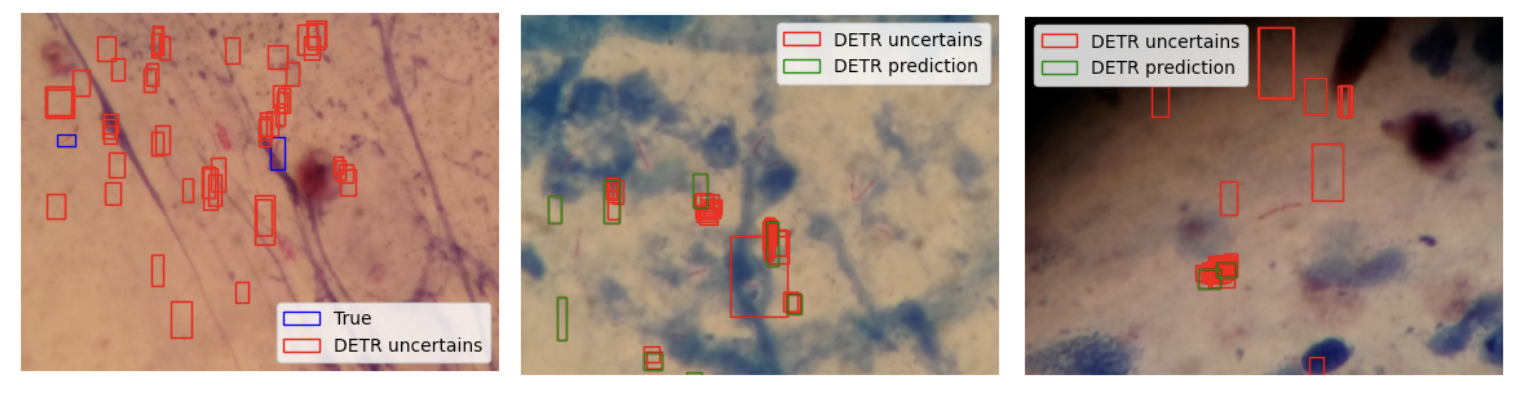
\includegraphics[width=1\linewidth]{figures/overtargeting.png}
    %     \caption{Example of overestimations in the model's predictions.
    %     The model predicts a large amount of bacilli spread apart while the ground truth only contains a few.
    %     }
    %     \label{fig:overtargeting}
    % \end{figure}
    
    
    % An image where all boxes overlap in one area would have a smaller value than one that is more spread apart. This gave us a function to rank images according to this 

    
    
    % The performance of our adaptive system was, again, evaluated using the performance metrics AP and AR at IoU thresholds of 0.3 and 0.5. This allowed us to measure the incremental improvement in the model’s performance as a result of the continuous learning process.
    

    % % With regards to 

    % % The following table summarises the structure and design of the experiments.
    
    % \todo[inline]{si tienes tiempo añade un diagrama detallando este proceso}


% \printbibliography
\end{document}